\chapter{Implementation and Evaluation}
\label{chap:implementation}

We implement a prototype of the recovery protocol to validate the design and demonstrate its
feasibility. The prototype is written in TypeScript and runs on Node.js, chosen for rapid
development and the availability of cryptographic libraries. While the prototype is not
optimized for production use, it faithfully implements the protocol described in
Chapter~\ref{chap:protocol} and serves as a reference implementation.

\section{System Architecture}
\label{sec:system-architecture}

The prototype consists of three main components: validators, clients, and a shared common
library. Figure~\ref{fig:system-architecture} illustrates the high-level architecture.

\begin{figure}[ht]
\centering
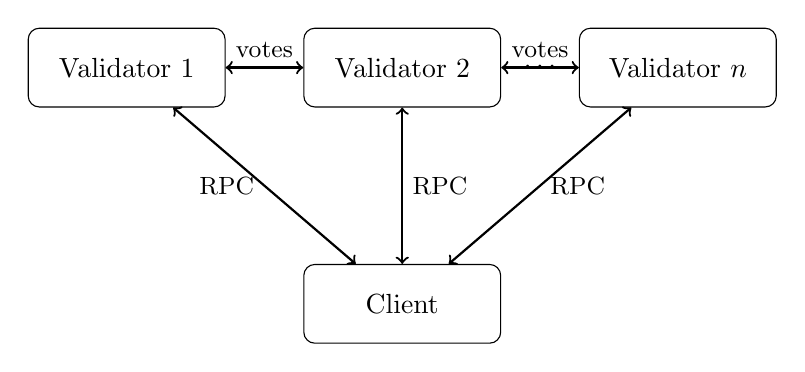
\begin{tikzpicture}[
    component/.style={draw, rounded corners, minimum width=2.5cm, minimum height=1cm, align=center},
    arrow/.style={->, thick},
    label/.style={font=\small}
]

% Validators
\node[component] (v1) at (0, 0) {Validator 1};
\node[component] (v2) at (3.5, 0) {Validator 2};
\node[component] (v3) at (7, 0) {Validator $n$};
\node at (5.25, 0) {$\cdots$};

% Client
\node[component] (client) at (3.5, -3) {Client};

% Arrows
\draw[arrow, <->] (client) -- (v1) node[midway, left, label] {RPC};
\draw[arrow, <->] (client) -- (v2) node[midway, right, label] {RPC};
\draw[arrow, <->] (client) -- (v3) node[midway, right, label] {RPC};

% Validator-to-validator
\draw[arrow, <->] (v1) -- (v2) node[midway, above, label] {votes};
\draw[arrow, <->] (v2) -- (v3) node[midway, above, label] {votes};

\end{tikzpicture}
\caption{System architecture showing validators communicating via vote propagation and clients
interacting with validators through JSON-RPC.}
\label{fig:system-architecture}
\end{figure}

\textbf{Validators.} Each validator runs as an independent HTTP server that exposes a JSON-RPC
endpoint. Validators maintain local state including account balances, nonces, and collected
votes. When a validator receives a transaction, it validates the request, signs a vote, and
broadcasts the vote to all other validators. Validators use the ethers.js library for
cryptographic operations including transaction parsing, signature verification, and vote signing.

\textbf{Clients.} The client library provides methods for sending transactions and initiating
recovery. Clients broadcast transactions to all validators in parallel and collect votes from
the responses. The client verifies each vote signature before counting it toward the quorum.
For recovery, clients query validators for the current account state and construct a recovery
transaction referencing an appropriate tip.

\textbf{Common Library.} Shared data structures and utility functions are defined in a common
module. This includes protocol constants (quorum sizes, recovery contract address), type
definitions (votes, certificates, account state), and cryptographic utilities (vote verification,
quorum counting).

\section{Implementation Details}
\label{sec:implementation-details}

\textbf{Transaction Format.}
The prototype uses standard Ethereum transaction format, leveraging the ethers.js library for
serialization and signature handling. Transactions are serialized as RLP-encoded hex strings
for network transmission. This design choice provides compatibility with existing Ethereum
wallets and signing tools, well-tested serialization code, and a familiar transaction structure
for developers. Recovery transactions are distinguished by their recipient address: the designated
recovery contract at \texttt{0x0...0100}. The tip transaction is embedded in the \texttt{data}
field as a serialized transaction, allowing validators to extract and verify it.

\textbf{Vote Structure and Signing.}
Votes contain five fields: the validator address, account address, nonce, serialized transaction
(or null for $\bot$), and signature. The signature is computed over a packed encoding of the
account address, nonce, and transaction hash (or zero hash for $\bot$):
\[
\mathsf{message} = \mathsf{keccak256}(\mathsf{account} \| \mathsf{nonce} \| \mathsf{txHash})
\]
This scheme allows efficient verification: given a vote, anyone can recover the signer's address
and verify it matches the claimed validator. Validators verify incoming votes against a known
validator set to prevent Sybil attacks.

\textbf{State Management.}
Each validator maintains two mappings: (1) account state, which maps addresses to
$(\mathsf{balance}, \mathsf{nonce}, \mathsf{pending}, \mathsf{finalised})$ tuples where the
\texttt{pending} flag indicates whether the account has an in-flight transaction; and (2) vote
storage, which maps $(\mathsf{address}, \mathsf{nonce})$ pairs to lists of received votes.
Validators store all votes to support certificate construction and recovery queries. When
processing votes, validators check for duplicates to prevent double-counting. For normal votes,
a validator accepts at most one vote per validator per nonce. For $\bot$ votes, the validator
may receive both a normal vote and a $\bot$ vote from the same validator (if the validator
initially voted for a transaction but later signed $\bot$ when no transaction achieved
notarization quorum).

\textbf{Network Communication.}
Communication between components uses JSON-RPC over HTTP. The prototype implements three RPC
methods: \texttt{eth\_sendRawTransaction} to submit a signed transaction and receive the
validator's vote; \texttt{submitVote} to propagate votes between validators; and
\texttt{eth\_getRecoveryInfo} to query the validator's view of an account's state including
the chain of certificates needed for recovery. The naming convention follows Ethereum's
JSON-RPC API where applicable, facilitating integration with existing tooling.

\textbf{Certificate Handling.}
Unlike the pseudocode which treats certificates as explicit objects passed between validators,
the prototype takes a simpler approach: validators implicitly form certificates by collecting
votes. When a validator accumulates $n-f$ votes for a nonce, it processes the certificate
inline. This design reduces message complexity-validators only broadcast individual votes,
not assembled certificates. The \texttt{getMaxQuorumCert} helper function extracts the
transaction with the most votes from a set of votes, implementing the certificate extraction
logic from Algorithm~\ref{alg:validator-recovery-cert}.

\textbf{Recovery Flow.}
The recovery implementation follows the protocol specification. First, the client detects a
potential lock when a transaction does not achieve finality quorum. The client then queries
multiple validators for recovery information and selects the response with the highest current
nonce. From this response, the client identifies the tip transaction: the last non-$\bot$
transaction in the certificate chain, or the last finalized transaction if all intermediate
nonces are $\bot$. Finally, the client constructs a recovery transaction with the tip embedded
in the data field and broadcasts it to collect votes as usual.

\section{Experimental Setup}
\label{sec:experimental-setup}

We evaluate the prototype using a local test network with configurable parameters. The default
configuration uses $n = 6$ validators with $f = 1$ Byzantine fault tolerance, giving a finality
quorum of $n - f = 5$ and a notarization quorum of $n - 3f = 3$.

\textbf{Test Scenarios.}
The test suite validates the protocol through a sequence of scenarios:

\begin{enumerate}
    \item \textbf{Normal operation}: A client sends a transaction that achieves finality quorum.
        All validators vote for the same transaction, the certificate is formed, and the
        transaction is finalized.

    \item \textbf{Conflicting transactions}: The client (simulating malicious behavior) sends
        conflicting transactions to different validator subsets. With 6 validators split 3-3,
        neither transaction achieves the finality quorum of 5, causing the account to lock.

    \item \textbf{Locked account rejection}: While locked, the client attempts a normal
        transaction at the next nonce. Validators reject this because the account's pending
        flag is set.

    \item \textbf{Recovery}: The client queries validators for recovery information, constructs
        a recovery transaction pointing to one of the conflicting transactions (which has
        notarization quorum), and successfully recovers the account.
\end{enumerate}

\textbf{Configuration Parameters.}
The prototype supports configuration through environment variables:
\begin{itemize}
    \item \texttt{N\_VALIDATORS}: Total number of validators (default: 6)
    \item \texttt{F\_BYZANTINE}: Maximum Byzantine validators (default: 1)
\end{itemize}

The implementation validates that $n \geq 5f + 1$ at startup, rejecting invalid configurations.

\section{Performance Evaluation}
\label{sec:performance-evaluation}

To quantify the overhead introduced by the recovery mechanism, we compare two
protocol variants under identical network conditions: \emph{Classic FastPay},
which implements the original protocol without recovery support, and
\emph{FastPay with Recovery}, which includes the full recovery mechanism
described in Chapter~\ref{chap:protocol}.

\subsection{Classic FastPay Implementation}

The classic variant strips the recovery-related code paths from the validator:
no bot voting, no notarisation quorum, and no recovery transaction handling.
When a validator receives a vote, it checks only whether the finality quorum
of $n - f$ votes has been reached for a single transaction at the current nonce.
If so, the transfer is executed and the nonce advances. If conflicting
transactions prevent any single transaction from reaching the quorum, the
account remains permanently locked---precisely the limitation that motivates
the recovery protocol.

To ensure a fair comparison, each protocol is configured with its
maximum tolerable~$f$ for a given~$n$:
\begin{itemize}
    \item Classic FastPay: $f = \lfloor(n-1)/3\rfloor$ (the standard $3f+1$ model)
    \item FastPay with Recovery: $f = \lfloor(n-1)/5\rfloor$ (the $5f+1$ model)
\end{itemize}
Both share the same network infrastructure (HTTP JSON-RPC), cryptographic
operations (ethers.js signing and verification), and client-side logic (broadcast
to all validators, collect votes). The only difference lies in the certificate
processing logic and the resulting finality quorum ($n - f$).

\subsection{Benchmark Methodology}

We measure two metrics: \emph{throughput} (finalized transactions per second)
and \emph{latency} (time from broadcasting a transaction to receiving
$n - f$ valid votes back from the validators).

\textbf{Setup.}
The benchmarks use $n = 6$ validators, each running as a separate operating
system process with its own HTTP JSON-RPC server. Validators communicate
via HTTP for both client requests and inter-validator vote propagation,
with $f$ set according to the protocol variant. All processes run on the
same machine to eliminate network variability while still parallelizing
cryptographic operations across CPU cores. All transaction signatures are
precomputed before each benchmark run so that the measurement phase captures
only protocol execution time. The latency timer resolves as soon as $n - f$
vote responses arrive from the validators.

\textbf{Benchmark~1: Happy-path throughput and latency.}
To measure the maximum achievable throughput, we use a separate account for
every transaction, removing the sequential nonce bottleneck. The offered load
increases across phases (10, 20, 40, 80, 120, 160~tx/s), with
each phase running for 10 seconds. We expect the latency to remain flat at low
load and spike once the system saturates, producing an L-shaped curve.

\textbf{Benchmark~2: Single-account sequential throughput.}
A single account sends transactions back-to-back (each transaction waits for
quorum before the next is submitted, due to nonce ordering). This measures the
sequential per-account throughput---the fastest rate at which one user can
finalize transactions.

\textbf{Benchmark~3: Recovery impact on throughput.}
A single account sends transactions at its maximum sequential rate. After
10~seconds of steady-state operation, the client equivocates by sending
conflicting transactions, locking the account. The client then immediately
initiates recovery and resumes normal transactions. Per-second throughput is
tracked as a time series to show that recovery causes at most a brief
interruption.

\subsection{Results}

\textbf{Happy-path throughput and latency.}
Figure~\ref{fig:bench1-latency} shows the latency as a function of
achieved throughput for both protocol variants. At low throughput, both
protocols achieve similar median latency (${\sim}5$--$8$\,ms). As the throughput
approaches the saturation point (${\sim}80$--$120$\,tx/s), latency increases by
several orders of magnitude---the characteristic L-shaped curve of a saturating
system. The 95th-percentile tail latency shows the same pattern. Both protocols
saturate at a similar point, demonstrating that the recovery mechanism adds
negligible overhead to the fast path.

\begin{figure}[ht]
\centering
\begin{tikzpicture}
\begin{axis}[
    xlabel={Throughput [tx/s]},
    ylabel={Latency [ms]},
    ymode=log,
    ymin=3,
    ymax=20000,
    ytick={5,10,50,100,1000,10000},
    yticklabels={5,10,50,100,1000,10000},
    width=0.85\textwidth,
    height=7cm,
    legend pos={north west},
    grid=major,
    legend cell align={left},
]
\addplot[color=TUMBlue, mark=*, thick]
    table[x=classic_tps, y=classic_median, col sep=tab] {data/bench1-latency.dat};
\addplot[color=TUMOrange, mark=square*, thick]
    table[x=recovery_tps, y=recovery_median, col sep=tab] {data/bench1-latency.dat};
\addplot[color=TUMBlue, mark=*, thick, dashed]
    table[x=classic_tps, y=classic_p95, col sep=tab] {data/bench1-latency.dat};
\addplot[color=TUMOrange, mark=square*, thick, dashed]
    table[x=recovery_tps, y=recovery_p95, col sep=tab] {data/bench1-latency.dat};
\legend{Classic (p50), Recovery (p50), Classic (p95), Recovery (p95)}
\end{axis}
\end{tikzpicture}
\caption{Latency vs.\ throughput. Solid lines show median, dashed lines show
95th percentile. Both protocols exhibit the L-shaped curve characteristic of a
saturating system.}
\label{fig:bench1-latency}
\end{figure}

\textbf{Single-account sequential throughput.}
Table~\ref{tab:bench2} compares the sequential throughput of both protocols
when a single account sends transactions back-to-back for 30~seconds.

\begin{table}[ht]
\centering
\caption{Single-account sequential throughput comparison ($n=6$).}
\label{tab:bench2}
\begin{tabular}{lcccc}
\toprule
\textbf{Protocol} & \textbf{Throughput [tx/s]} & \textbf{Median [ms]} & \textbf{Mean [ms]} & \textbf{p95 [ms]} \\
\midrule
Classic FastPay & 105.8 & 4.4 & 4.8 & 6.9 \\
FastPay with Recovery & 90.2 & 5.9 & 6.2 & 8.2 \\
\bottomrule
\end{tabular}
\end{table}

The results confirm that the recovery mechanism introduces minimal overhead on
the fast path: the additional code paths for bot voting and recovery validation
are never triggered during normal operation and do not measurably affect
per-transaction latency.

\textbf{Recovery impact on throughput.}
Figure~\ref{fig:bench3-timeseries} shows the per-second throughput of a single
account over time. After 10~seconds of steady-state operation, the client
equivocates, locking the account. Recovery is initiated immediately, and normal
transactions resume. The throughput timeline shows that recovery causes only a
brief interruption in the equivocation second, after which throughput returns to
the pre-equivocation level.

\begin{figure}[ht]
\centering
\begin{tikzpicture}
\begin{axis}[
    xlabel={Time [s]},
    ylabel={Throughput [tx/s]},
    ymin=0,
    width=0.85\textwidth,
    height=6cm,
    grid=major,
    legend cell align={left},
    legend pos={south east},
]
\addplot[color=TUMBlue, thick, mark=none]
    table[x=timeSec, y=throughput, col sep=tab] {data/bench3-timeseries.dat};
\draw[dashed, TUMOrange, thick] (axis cs:10.0,0) -- (axis cs:10.0,100)
    node[above, font=\footnotesize] {equivocation};
\draw[dashed, TUMGreen, thick] (axis cs:10.5,0) -- (axis cs:10.5,100)
    node[above, font=\footnotesize] {recovery};
\legend{FastPay with Recovery}
\end{axis}
\end{tikzpicture}
\caption{Per-second throughput during equivocation and recovery. The vertical
dashed lines mark the equivocation and recovery events. Throughput recovers
immediately after the recovery transaction is finalized.}
\label{fig:bench3-timeseries}
\end{figure}

